%%%%%%%%%%%%%%%%%%%%%%%%%%%%%%%%%%%%%%%%%
% Journal Article
% LaTeX Template
% Version 2.0 (February 7, 2023)
%
% This template originates from:
% https://www.LaTeXTemplates.com
%
% Author:
% Vel (vel@latextemplates.com)
%
% License:
% CC BY-NC-SA 4.0 (https://creativecommons.org/licenses/by-nc-sa/4.0/)
%
% NOTE: The bibliography needs to be compiled using the biber engine.
%
%%%%%%%%%%%%%%%%%%%%%%%%%%%%%%%%%%%%%%%%%

%----------------------------------------------------------------------------------------
%   PACKAGES AND OTHER DOCUMENT CONFIGURATIONS
%----------------------------------------------------------------------------------------
\documentclass[
    a4paper, % Paper size, use either a4paper or letterpaper
    10pt, % Default font size, can also use 11pt or 12pt, although this is not recommended
    unnumberedsections, % Comment to enable section numbering
    twoside, % Two side traditional mode where headers and footers change between odd and even pages, comment this option to make them fixed
]{LTJournalArticle}

\usepackage[utf8]{inputenc}
 % BibLaTeX bibliography file
\usepackage{etoolbox}
\addbibresource{reference.bib}
\usepackage{adjustbox}
\usepackage{indentfirst} 
\usepackage{graphicx} % 包含图形
\usepackage{subcaption} % 子图
\usepackage{amsmath}
\usepackage{tcolorbox}
 % A shortened article title to appear in the running head, leave this command empty for no running head
\linespread{2}
\footertext{\textit{Class Article of "Fundamentals of Quantum Information"} (2024- 06-10)} % Text to appear in the footer, leave this command empty for no footer text
\makeatletter
\preto{\@enddocumenthook}{\printbibliography}
\newcommand{\rmnum}[1]{\romannumeral #1}
\newcommand{\Rmnum}[1]{\expandafter\@slowromancap\romannumeral #1@}
\makeatother
\setcounter{page}{1} % The page number of the first page, set this to a higher number if the article is to be part of an issue or larger work
\newtcolorbox{mathbox}[1][]{%
    colback=white, % 背景颜色
    colframe=blue!75!black, % 边框颜色
    opacityframe=0, % 边框透明度
    sharp corners, % 边框为直角
    boxrule=0.5mm, % 边框宽度
    left=5pt, % 左边距
    right=5pt, % 右边距
    top=5pt, % 顶部边距
    bottom=5pt, % 底部边距
    #1 % 允许自定义参数
}
\renewcommand{\baselinestretch}{1.2} % Adjust the line spacing

%----------------------------------------------------------------------------------------
%   TITLE SECTION
%----------------------------------------------------------------------------------------

\title{A Comparative Analysis of the MWPM Surface Codes} % Article title, use manual lines breaks (\\) to beautify the layout

% Authors are listed in a comma-separated list with superscript numbers indicating affiliations
% \thanks{} is used for any text that should be placed in a footnote on the first page, such as the corresponding author's email, journal acceptance dates, a copyright/license notice, keywords, etc
\author{
    Zicheng Yang$^1$, Yuheng Ma$^2$, Yiming Xiao$^3$, Zikang Lv$^4$
}

% Affiliations are output in the \date{} command
\date{\footnotesize\ $^1$School of physics, ZheJiang University \\ $^2$School of computer science and technology, ZheJiang University \\  $^3$School of computer science and technology, ZheJiang University \\  $^4$School of physics, ZheJiang University \\ (\today)}

% Full-width abstract
\renewcommand{\maketitlehookd}{%
    \begin{abstract}
        \noindent Nowadays more and more decoders for quantum error correction are published, many of which are potential in surface code decoding. We compared the decoding performance of different decoders from some vital criteria. Our simulations reveal the blossom algorithm's performance in various quantum memory scales and physical error rate, demonstrating an error threshold of approximately 0.104. The Blossom Algorithm may not distinguish in time complexity compared to some contemporary methods. However, its higher error threshold presents a strategic advantage for specific quantum computing tasks. At the end we conclude with a trade-off of decoders in three aspects: time consuming, error threshold and logical error rate. We anticipate the emergence of a decoder that excels across these three dimensions, which can be the winner. \
         For more information, please visit our official GitHub repository at \url{https://github.com/Winfred666/SurfaceCode-MWPMDecoder.git}.

    \end{abstract}
}

%----------------------------------------------------------------------------------------

\begin{document}

\maketitle % Output the title section

%----------------------------------------------------------------------------------------
%   ARTICLE CONTENTS
%----------------------------------------------------------------------------------------

\section{\Rmnum{1}. Introduction}
With the popularity of quantum computing spreading in the investors and researchers, quantum error correcting has also been much under scrutiny. Though in the early time, people have the skepticism that weather quantum computing can keep and manipulate a quantum state error-free for a long time \cite{1}, the development of quantum error correction making it more optimistic.

Among so many prospective codes of quantum error correcting, the most promising classes is the surface code, which is proposed by Alexei Kitaev in 1997 \cite{2}. The topological concept of the surface code or toric code is to encode the qubit in a 2D lattice of physics qubits system which has some specific boundary condition \cite{3}. In this case, we can influence and correct a wide range of qubits by applying a given way on the torus. Although challenges of fabricating a large-scale quantum memory still exist, the progresses on experimental advances in recent years give us hope to make it a reality \cite{4}\cite{5}.

Another significant period of a quantum error correcting task is to decode. It is natural that we want to find an optimal solution to figure out the most probably error and correct it for every given measurement, which is called the Maximums Like Algorithm. But it seems unpractical for its exponential operation time \cite{6}, so how to balance between performance and running time of the algorithm becomes the priority. A lot of solution has been designed to solve such problems, such as the graph algorithm and neural network \cite{7}.

In this paper, we will take an insight of a kind of graph algorithm, the Blossom Algorithm. As well as we will compare it with other decoder algorithm from multiple dimensions.

%------------------------------------------------

\section{\Rmnum{2}. Background of Quantum Error Correction}

A standard error correction usually consists of four step \cite{7}:
\begin{enumerate}
    \item \textbf{Encode} : encode the logical quantum state to another defined state, for example:
    \begin{center}
    $\vert \psi \rangle= \alpha \vert 0 \rangle +\beta \vert 1 \rangle \rightarrow \vert \psi_{E} \rangle=\alpha \vert 000 \rangle +\beta \vert 111 \rangle$
    \end{center} 
    \item \textbf{Detect} : detect the quantum errors by measurement
    \item \textbf{correct} : correct those errors and decode the qubits to get the corresponding logical state
    \item \textbf{compute} : compute logical operations on the state by redefining a universal gate set on the code.
\end{enumerate}
Here we will focus on the first three steps and outline our work by the following steps:
\begin{enumerate}
    \item \textbf{Introduce errors}
    \item \textbf{Plot syndromes}
    \item \textbf{Match the syndromes}
    \item \textbf{Get the result}
\end{enumerate}

\subsection{A. toric code}

For a better understanding of the toric code, we assume a L$\times$L lattice, where every single qubit lives on the stage, so we have $L^2$ qubits. The stabilizer group of toric code is generated by two types of operator $A_s$ and $B_p$ \cite{8}:
\begin{center}
$A_s = \bigotimes X_q,B_p = \bigotimes Z_q$
\end{center}
The X and Z are the Pauli matrix the Hamiltonian of the system is the linear combination of the tow operator:
\begin{center}
$H = -A_s-B_p$
\end{center}
We show the stabilizer and the lattice in Figure 1.
\begin{figure} % Single column figure
    \setlength{\abovecaptionskip}{0.cm} %调整标题上方的距离   
    \setlength{\abovecaptionskip}{0.cm} 
    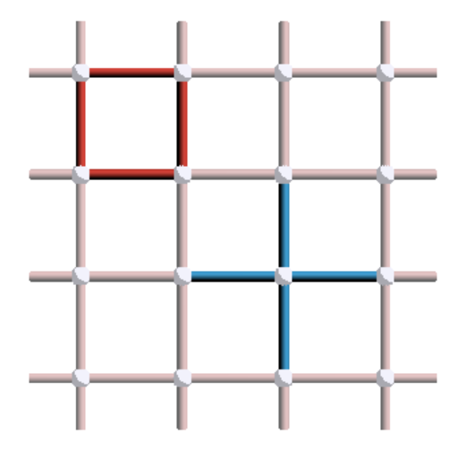
\includegraphics[width=\linewidth]{img/figure 1.png}
    \caption{An illustration of the lattice. The unit marked by the red line or the blue line shows the $A_s$ operator and $B_p$ operator respectively}
    \label{fig:tcanther}
\end{figure}

\subsection{B. Quantum Error}

Generally speaking, the noisy and environment disturbance is inevitable in real quantum system. It is impossible for us to clarify the procedure of the coupling between the system and the environment. But in fact, we can ease the challenge by simplifying all the quantum errors into two types of error:
\begin{center}
Bit-flips error:$\vert \psi \rangle \rightarrow \hat{X} \vert \psi \rangle$
\end{center}
\begin{center}
Phase-slip error:$\vert \psi \rangle \rightarrow \hat{Z} \vert \psi \rangle$
\end{center}
The X error and the Y error are the fundamental mode of quantum error and they can appear at the same time, which we call Y error. In this paper, we assume that each error has the same probability $p/3$ to occur(in the code we implement ,the p is 0.15).
\begin{figure}[htbp] % Single column figure 
    \centering  %使图片居中显示
    \vspace{-0.8cm}   %调整图片与上文的垂直距离  
    \setlength{\abovecaptionskip}{0.cm} %调整标题上方的距离   
    \setlength{\abovecaptionskip}{0.cm} %调整标题下方的距离     
    \setlength{\belowdisplayskip}{3pt}  
    \begin{subfigure}[b]{0.45\linewidth}
        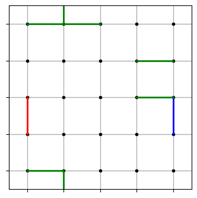
\includegraphics[width=\linewidth]{img/figure 2.png}
        \caption{errors occur}
        \label{fig:subfig1}
    \end{subfigure}
    \hfill
    \begin{subfigure}[b]{0.45\linewidth}
        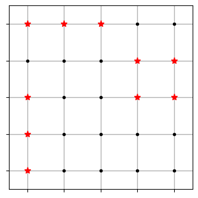
\includegraphics[width=\linewidth]{img/figure 2.1.png}
        \caption{detect syndromes.}
        \label{fig:subfig2}
    \end{subfigure}
    \vskip\baselineskip
    \begin{subfigure}[b]{0.45\linewidth}
        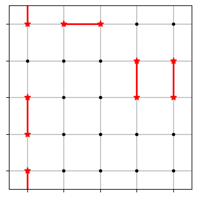
\includegraphics[width=\linewidth]{img/figure 2.2.png}
        \caption{matching}
        \label{fig:subfig3}
    \end{subfigure}
    \hfill
    \begin{subfigure}[b]{0.45\linewidth}
        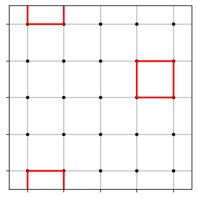
\includegraphics[width=\linewidth]{img/figure 2.3.png}
        \caption{decoder}
        \label{fig:subfig4}
    \end{subfigure}
    \caption{the procedure of an error correction. (a)-(d) shows the different stage respectively}
    \label{fig:fourfigs}
    \vspace{-0.4cm}
\end{figure}
\subsection{C. Decoder}
As shown in Figure 2(a)-(d), when a series of errors happen and we detect this error by the measurement and collect all the syndromes. The task of decoder is to restore the most possible error. The green line ,red line and blue line in Figure 2(a) indicate the X error ,Z error and Y error. It is showed in the figure 2(b) that we detect these error with the measurement we mention above. The next step and the most challenging part is to match the syndromes and decode them to get result. We definitely hope what we get is trivial, but sometimes the logical error or the non-trivial result is inevitable due to the limitation of decoder algorithm \cite{9}. In the next section, we will introduce the Blossom Algorithm and test its logical error rate and compare it with other decoder algorithm.

%------------------------------------------------

\section{\Rmnum{3}. Blossom Algorithm}

The Blossom algorithm is the core of MWPM, and the step of building the syndrome graph from lattice using local dijkstra, and the way to recover path after matching the two defects, are ignored here. Interested readers can refer to the original PyMatching1.0 paper for more details.
Here,we implement this algorithm,which is first proposed by Edmonds in 1965.Edmond's idea requires $O(n^2m)$ times,where n is the number of nodes in the graph and m is the number of edges.The Blossom Algorithm has been developed with the time and different improvement has been conducted.It is impossible for us to cover all the creative ideas.Before we discuss the kind of minimum weight matching Blossom Algorithm,we first get an insight of the oldest Blossom Algorithm.

\begin{enumerate}
    % \item \textbf{Graph Representation}: First, you should represent the problem as a graph $G=(V,E)$, where V is the set of vertices and E is set of edges with associated weights, as shown in Figure 3 where each yellow ball represents the vertices and the segment represents the edge which has different weight.
    % \begin{figure} % Single column figure
    % \setlength{\abovecaptionskip}{0.cm} %调整标题上方的距离   
    % \setlength{\abovecaptionskip}{0.cm} 
    % 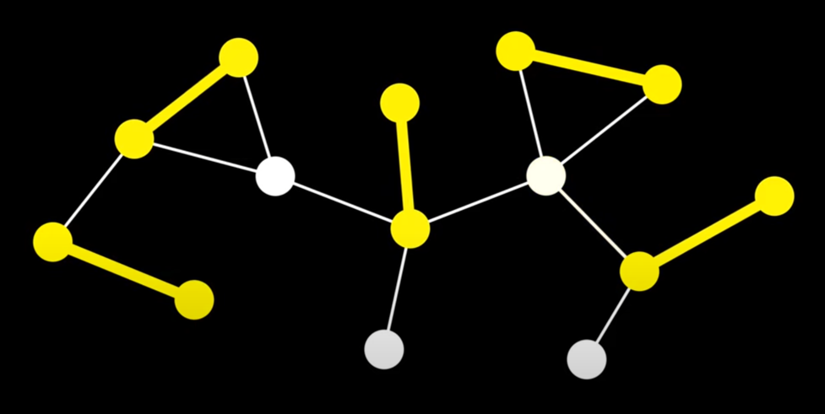
\includegraphics[width=\linewidth]{img/blossom algorithm 1.png}
    % \caption{An illustration of the graph. The balls represent the vertices and some are matched with each other and some are free}
    % \label{fig:tcanther}
    % \end{figure}
    \item \textbf{Augmenting Paths}: And then, an augmenting path is required. Like branches on a tree, an augmenting path is an alternating sequence of matched and unmatched edges, where the first and the last vertex is exposed, as shown in Figure 4(a). It can improve the size of the current matching by switching the matched and unmatched edges, as shown in Figure 4(b). And the process of matching can repeat until no free vertices are left, at which point, we know the matching is maximum, as shown in Figure 4(c). We can prove that: 
    \begin{center}
        contains an augmenting path $\leftrightarrow $ matching is not maximum
    \end{center}
    \begin{figure}[htbp] % Single column figure 
    \centering %使图片居中显示
    \vspace{0cm} %调整图片与上文的垂直距离  
    \setlength{\abovecaptionskip}{0.cm} %调整标题上方的距离   
    \setlength{\belowcaptionskip}{0.cm} %调整标题下方的距离  
    \setlength{\belowdisplayskip}{3pt} %调整标题与下文的距离
    \begin{subfigure}[b]{0.45\linewidth}
        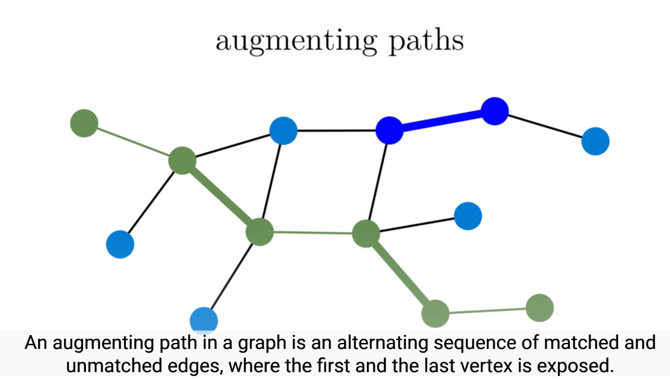
\includegraphics[width=\linewidth]{img/blossom algorithm 2.png}
        \caption{augmenting path}
        \label{fig:subfig1}
    \end{subfigure}
    \hfill
    \begin{subfigure}[b]{0.45\linewidth}
        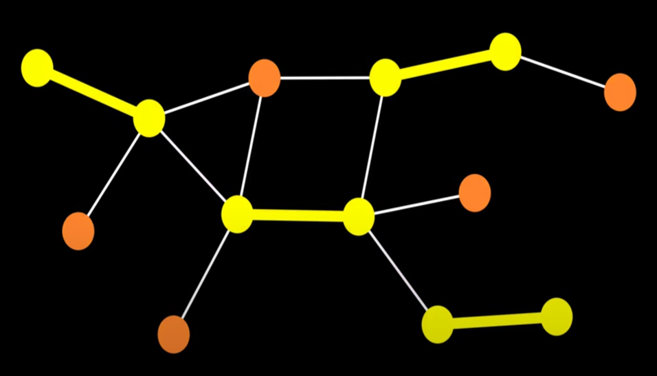
\includegraphics[width=\linewidth]{img/blossom algorithm 3.png}
        \caption{switch the edges}
        \label{fig:subfig2}
    \end{subfigure}
    \vskip\baselineskip
    \begin{subfigure}[b]{0.9\linewidth}
        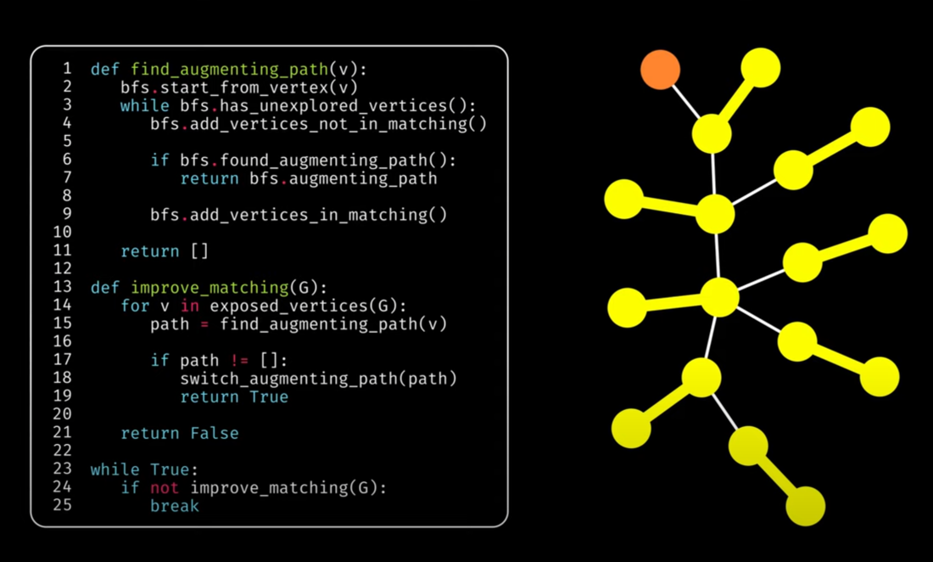
\includegraphics[width=\linewidth]{img/blossom algorithm 6.png}
        \caption{the blossom algorithm}
        \label{fig:subfig3}
    \end{subfigure}
    \vskip\baselineskip
    \begin{subfigure}[b]{0.45\linewidth}
        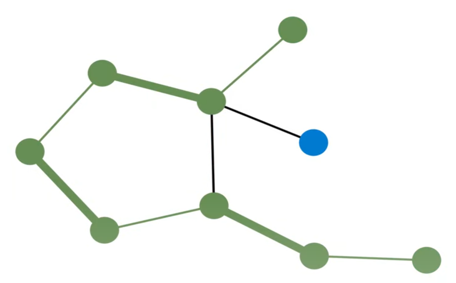
\includegraphics[width=\linewidth]{img/blossom algorithm 4.png}
        \caption{blossom}
        \label{fig:subfig4}
    \end{subfigure}
    \hfill
    \begin{subfigure}[b]{0.45\linewidth}
        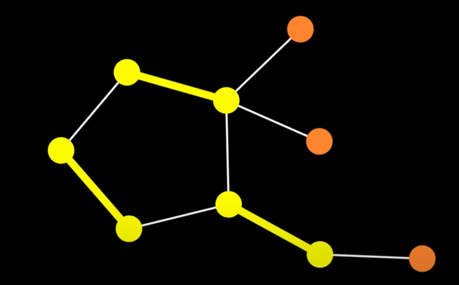
\includegraphics[width=\linewidth]{img/blossom algorithm 5.png}
        \caption{failed blossom}
        \label{fig:subfig5}
    \end{subfigure}
    \caption{the basic concepts of blossom algorithm}
    \label{fig:threefigs}
\end{figure}
    \item \textbf{Blossoms}: But things don't always go well. When there is a blossom, a cycle containing an odd number of “pseudo nodes”, where a pseudo node is either a vertex or another blossom, the algorithm fails, as shown in Figure 4(d) and 3(e). We can see that since the augmenting path is longer than the shortest path, it is not found.
    \item \textbf{Blossom Contraction and Expansion}: In this case, When an odd-length cycle (blossom) is detected, we should contract it into a single vertex, simplifying the problem and after finding a matching, expand the blossoms back to update the matching accordingly. The Figure 5(a)-(d) show the solution when a blossom is detected step by step.
    \begin{figure}[htbp] % Single column figure 
    \centering  %使图片居中显示
    \vspace{0cm}   %调整图片与上文的垂直距离  
    \setlength{\abovecaptionskip}{0.cm} %调整标题上方的距离   
    \setlength{\abovecaptionskip}{0.cm} %调整标题下方的距离     
    \setlength{\belowdisplayskip}{3pt}  
    \begin{subfigure}[b]{0.45\linewidth}
        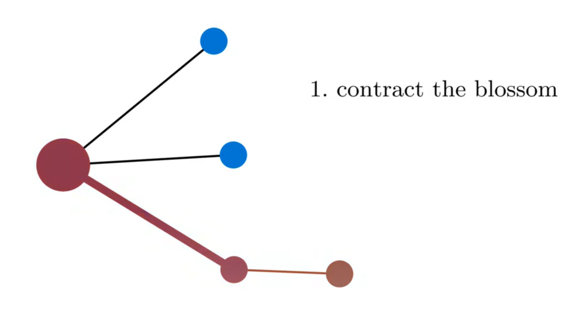
\includegraphics[width=\linewidth]{img/blossom algorithm 8.1.png}
        \caption{contract the blossom}
        \label{fig:subfig1}
    \end{subfigure}
    \hfill
    \begin{subfigure}[b]{0.45\linewidth}
        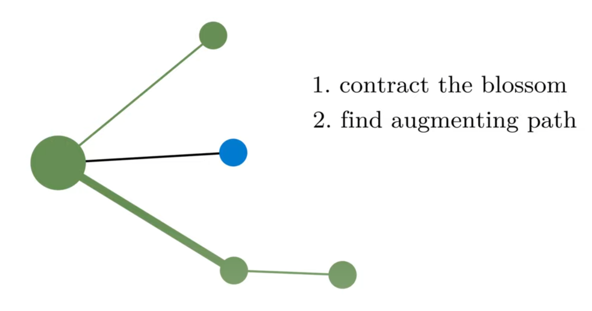
\includegraphics[width=\linewidth]{img/blossom algorithm 8,2.png}
        \caption{find augmenting path}
        \label{fig:subfig2}
    \end{subfigure}
    \vskip\baselineskip
    \begin{subfigure}[b]{0.45\linewidth}
        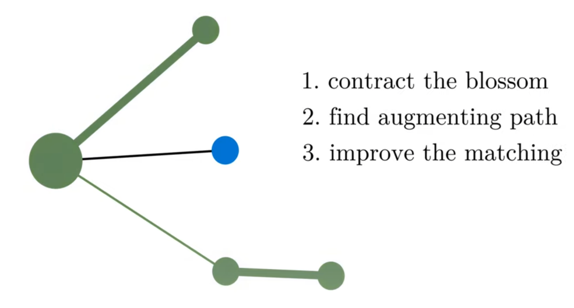
\includegraphics[width=\linewidth]{img/blossom algorithm 8.3.png}
        \caption{improve the matching}
        \label{fig:subfig3}
    \end{subfigure}
    \hfill
    \begin{subfigure}[b]{0.45\linewidth}
        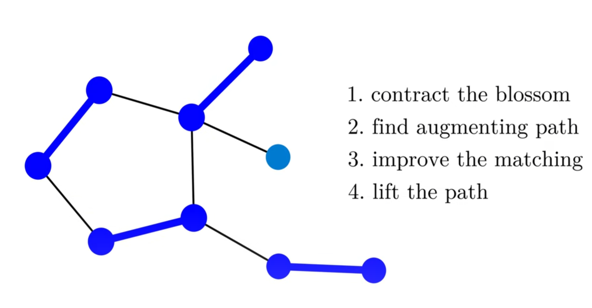
\includegraphics[width=\linewidth]{img/blossom algorithm 8.4.png}
        \caption{lift the path}
        \label{fig:subfig4}
    \end{subfigure}
    \caption{the contraction and expansion of blossoms. (a)-(d) shows the different step respectively}
\end{figure}
    \item \textbf{Iterative Process}: Finally, repeat the search for augmenting paths, contraction, and expansion until no more augmenting paths can be found. The whole process and code is presented in Figure 6.
\begin{figure} % Single column figure
    \setlength{\abovecaptionskip}{0.cm} %调整标题上方的距离   
    \setlength{\abovecaptionskip}{0.cm} 
    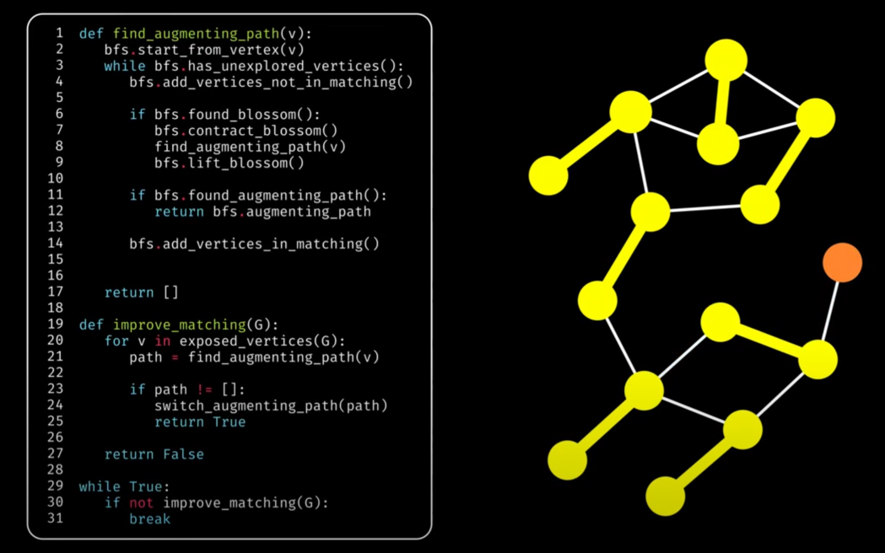
\includegraphics[width=\linewidth]{img/blossom algorithm 9.png}
    \caption{the whole process and the code}
\end{figure}
\end{enumerate} 
The minimum weight perfect matching algorithm is originated from the initial idea,
but it has some improvement to handle with the practical problems, because there are \emph{weight} in our syndrome graph!
Thus, we need a more complicated derived algorithm to solve our problem: Blossom V.
The implementation of the algorithm is the following:for every vertex $i$,it has a weight $l(i)$ and every edge is a coupling of the vertices $i,j$,it meets the condition:$w(i,j) \leq l(i)+l(j)$.Every perfect minimum weight matching,the sum of the weight edge is:
\begin{center}
\begin{align*}
    \text{val}(M) &= \sum_{(u,v)\in M}w(u,v) \\
    &\leq \sum_{(u,v)\in M}(l(u)+l(v)) \\
    &\leq \sum_{i=1}^{n}l(i)
\end{align*}
\end{center}
Defining $z_u$ as the vertex labeling of $u$, and we also define $e(u,v)$ an equality edge if $(z_u+z_v=weight(e))$, and at this time the edge labeling of edge is called $z_e$. It requires $z_e=z_u+z_v-weight(e)=0$.
The augmenting path composed of "equality edges" is continuously expanded, and since all the edges used for expansion are "equality edges", the final maximum weight perfect matching obtained is still all "equality edges".
In Figure 7, we demonstrate the whole process of this algorithm in detail. It consists of four steps \cite{10}:
\begin{enumerate}
    \item \textbf{Grow}: If edge $(u,v)$ is tight, $l(u) = + $and $l(v) = \emptyset$ then the tree to which $u$ belongs can be "grown" by acquiring node $u$ and the corresponding matched node, as shown in the Figure 7(a)
    \item \textbf{Augment}: If edge $(u,v) $ is tight, $l(u) = l(v) = + $ and $u,v$ belong to different trees then the cardinality of matching $x$ can be increased by "flipping" variable $x_e$ for edges $e$ along the path connecting the roots of the two trees, as shown in Figure 7(b). All nodes in the trees become free.
    \item \textbf{Shrink}: If edge $(u,v) $ is tight, $l(u) = l(v) = + $ and $u,v$ belong to the same tree then there is cycle of odd length that can be shrunk to a blossom, as shown in Figure 7(c). The dual variable for this new blossom is set to 0.
    \item \textbf{Expand}: If node $v$ is a blossom with $y_e = 0$ and $l(v) = -$ then it can be expanded(Fig.7(d)).
\begin{figure} % Single column figure
    \setlength{\abovecaptionskip}{0.cm} %调整标题上方的距离   
    \setlength{\abovecaptionskip}{0.cm} 
    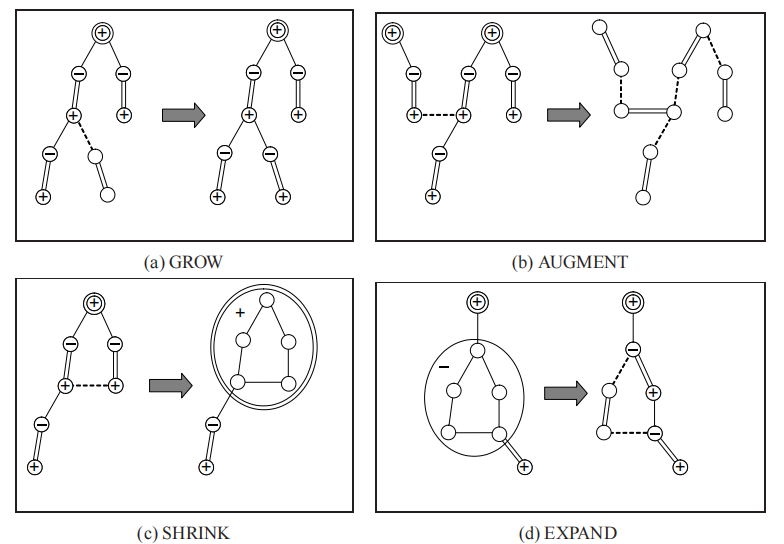
\includegraphics[width=\linewidth]{img/minimum weight.png}
    \caption{An illustration of the minimum weight perfect matching}
\end{figure}
\end{enumerate}
    The $u^-$ represents odd vertex in an alternating tree, while the $u^+$ represents the even vertex in an alternating tree and $u^{\emptyset}$ represents an vertex not in any alternating tree.

\section{\Rmnum{4}. Cellular Automation Decoder}
    Besides the Blossom Algorithm, we also get an insight of another decoder, the Cellular Automation Decoder. It offers a dynamical approach to decoding, while others pay attention to the graph problem. The CA decoder draws inspiration from statistical mechanics and field theories, which makes it more “physical” and natural. The whole system can be compared to a dissipative dynamical system driven away from equilibrium. Here we give a brief description of $\phi$-automation decoder that drives the system by Coulomb-like potential \cite{11}: 
\begin{enumerate}
    \item \textbf{Anyons Creation:} When errors occur, 'anyons' (or 'syndromes' we have mentioned in the passage) emerge at the ends of error strings.
    \item \textbf{Field Update Rule:} For each cell $\xi \in \Lambda(lattice)$, the field value at $\xi$, denoted by $\phi(\xi)$, is updated in parallel by taking the average of the field values at all neighboring cells $\xi'$ and adding the charge $q(\xi)$ if there is an anyon present at cell $\xi$. This can be expressed as: $$\phi(\xi) = \mathop{avg}\limits_{<\xi',\xi>}phi(\xi')+q(\xi)$$
    \item \textbf{Anyon Update Rule:} For each cell $x \in V(vertex)$, if there is an anyon present $(i.e.,q(x)\neq 0)$, then with $p=0.5$, the anyon moves to the neighboring cell y that has the highest local field value $\phi(y)$.
    \item \textbf{Iteration Continuation:} If anyons are still present after the updates, increase the sequence counter $\tau$ by 1 and repeat the steps above.
    \item \textbf{Termination Condition:} The process continues iteratively until there are no more anyons to move, indicating that the error syndromes have been resolved.
\end{enumerate}

\section{\Rmnum{5}. Test and result}
There is two critical parameter to evaluate the performance of a decoder:the error threshold and the time complexity.

However, One pitfall about test set of surface code is the usage of noisy model.
Though depolarizing noise model is the best one to simulate the real condition, 
most of the test program just generate only bit-flip errors to test the decoder.
So in \ref{fig:errorate2} we translate osur physical error rate
to the unit of commonly used one.

\begin{figure}[htbp] % Single column figure 
    \centering %使图片居中显示
    \vspace{0cm} %调整图片与上文的垂直距离  
    \setlength{\abovecaptionskip}{0.cm} %调整标题上方的距离   
    \setlength{\belowcaptionskip}{0.cm} %调整标题下方的距离  
    \setlength{\belowdisplayskip}{3pt} %调整标题与下文的距离
    \begin{subfigure}[b]{0.9\linewidth}
        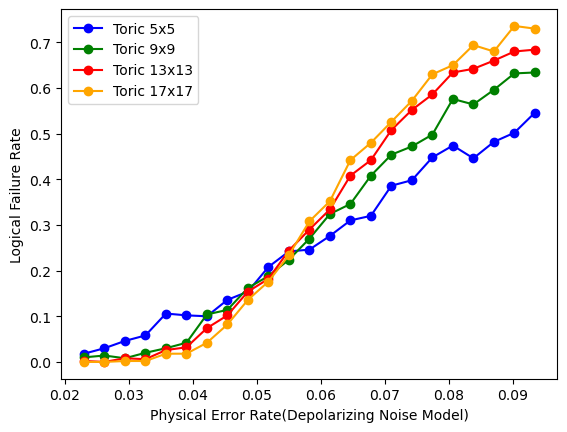
\includegraphics[width=\linewidth]{img/errorThres.png}
        \caption{}
        \label{fig:errorrate1}
    \end{subfigure}
    \hfill
    \begin{subfigure}[b]{0.9\linewidth}
        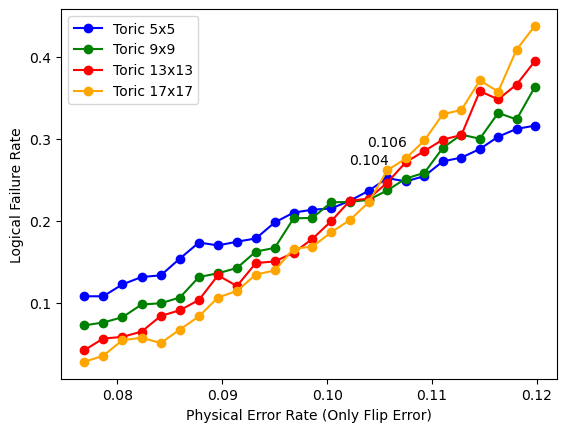
\includegraphics[width=\linewidth]{img/errorThres2.png}
        \caption{Error threshold of different decoders. (b) is more precise than (a) and use a more common unit.}
        \label{fig:errorate2}
    \end{subfigure}
    \caption{}
    \end{figure}


    In this part, we will show our results and compare different decoders with their error threshold and time complexity. You can see more details in our github website, here, we just give a brief introduction.
    The error threshold is a critical parameter in the design and implementation of fault-tolerant quantum computation. It is related to the threshold theorem, which states that arbitrarily long quantum computations are reliable below a specific error rate that varies with the quantum decoders we use. Above the specific error rate, the reliability of the quantum computation rapidly deteriorates, making it impossible to conduct a fault-tolerant quantum computation.
    Figure 8(a)-(b) shows the logical error rate varying with the phase-flip and bit-flip error rate under the noise model respectively. For four different scale quantum memories, we set up 25 different groups of error rates, each group of error rates for 500 simulation tests, and calculate the logic error rate. We can calculate the error threshold by recording the intersection of four lines. And it shows the error threshold is about 0.104. 
    

    For time complexity, we find our implementation using Blossom V very slow.
    Though we use local dijksra to build syndrome graph (see in Pymatching refer papers) ,
    which set a parameter M, and defects node will stop connecting with other nodes when its degree is larger than M.
    However,we just turn the time complexity from $O(n^3logn)$ \cite{12} to $O(n^2Mlogn)$, and there are risks of low accuracy.

    Luckily, in 2023 , Pymatching2.0, the new library use "sparse blossom algorithm", which has an amortize time of $O(n)$ and high accuracy.

    The comparison of time tested by us is shown in \ref{fig:time1} and \ref{fig:time2}. 
    
    \begin{figure}[htbp] % Single column figure 
        \centering %使图片居中显示
        \vspace{0cm} %调整图片与上文的垂直距离  
        \setlength{\abovecaptionskip}{0.cm} %调整标题上方的距离   
        \setlength{\belowcaptionskip}{0.cm} %调整标题下方的距离  
        \setlength{\belowdisplayskip}{3pt} %调整标题与下文的距离
        \begin{subfigure}[b]{0.9\linewidth}
            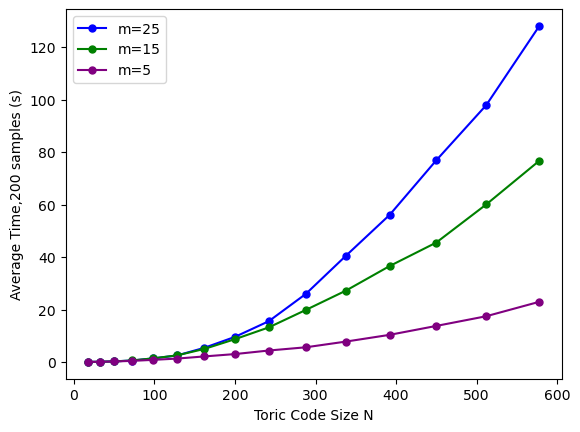
\includegraphics[width=\linewidth]{img/timespend_ours.png}
            \caption{}
            \label{fig:time1}
        \end{subfigure}
        \hfill
        \begin{subfigure}[b]{0.9\linewidth}
            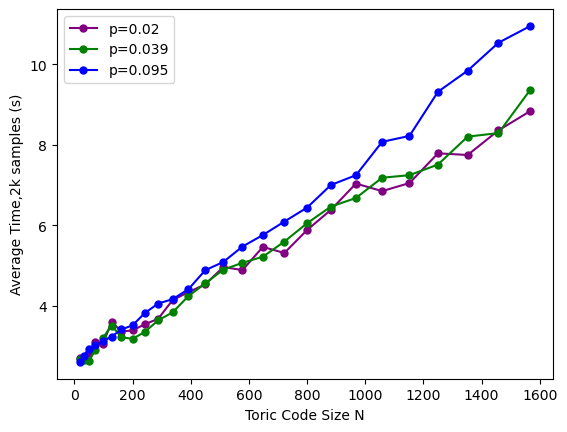
\includegraphics[width=\linewidth]{img/timespend_pymatch.png}
            \caption{}
            \label{fig:time2}
        \end{subfigure}
        \caption{Time complexity of (a) PyMatching1.2(our implementation) and (b) Pymatching2.0}
    \end{figure}

%------------------------------------------------
\begin{table}[h]
    \caption{Time complexity of different decoders\\(N is physical qubit number)}
    \centering
    \begin{adjustbox}{max width=\columnwidth}
    \begin{tabular}{>{\raggedright\arraybackslash}p{0.6\columnwidth} >{\raggedright\arraybackslash}p{0.4\columnwidth}}
        \toprule
        Decoder & Time Complexity \\
        \midrule
        MWPM(original) & $O(n^3logn)$ \\
        MWPM(M-local-dijkstra) & $O(n^2Mlogn)$ \\
        MWPM(sparse blossom) & $O(n)$ \\
        Cellular Automaton & $O(n^2)$ \\
        Union Find & $O(n)$ \\
        \bottomrule
    \end{tabular}
    \end{adjustbox}
\end{table}


\section{\Rmnum{6}. Conclusion}

%----------------------------------------------------------------------------------------
%    REFERENCES
%----------------------------------------------------------------------------------------
\printbibliography
%-------------------{}---{}------------------------------------------------------------------

\end{document}
